% !TeX encoding = UTF-8
\documentclass{beamer}
\usepackage{tikz}
\usepackage[utf8]{inputenc}
\usepackage[spanish]{babel}
\usepackage{graphicx}
\usepackage{smartdiagram}
\usepackage{qtree}
\usepackage{listings}
\usetheme{metropolis}
\usepackage{fontawesome}

\smartdiagramset{set color list={yellow!50,orange!50,red!50,yellow!30,orange!30,red!30}}



\usepackage{graphicx}

\usebackgroundtemplate
{
	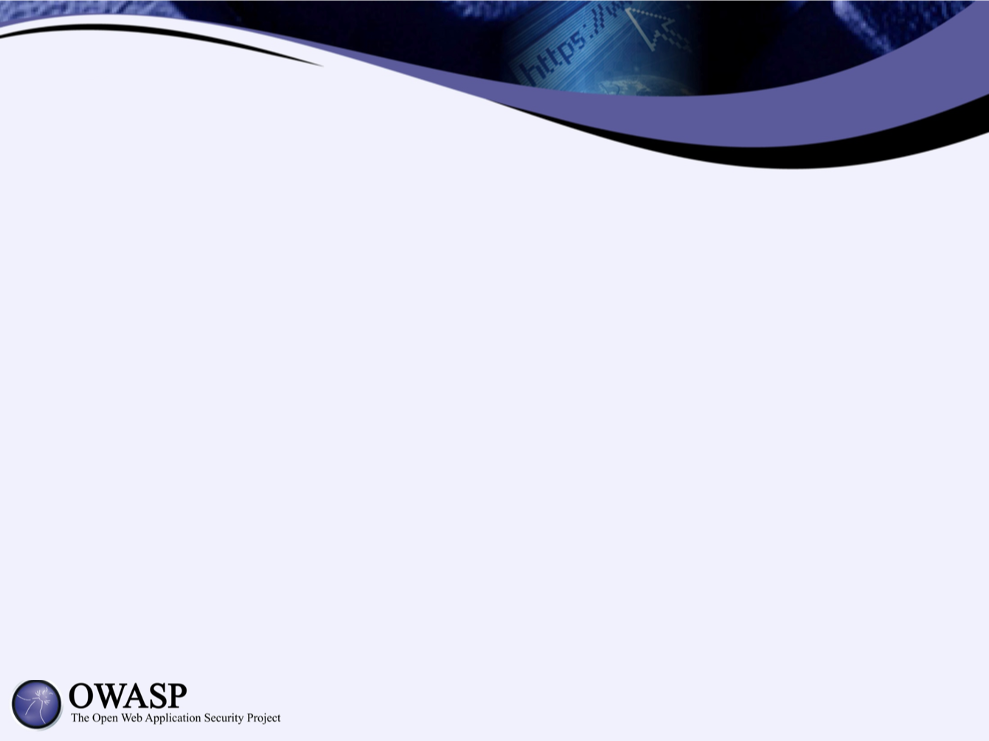
\includegraphics[width=\paperwidth]{Images/fondowasp}%
}



\title{Seguridad 101 JavaEE - OWASP Top 10}
\author{Víctor Orozco - @tuxtor}
\institute{Nabenik}
\date{\today}
\begin{document}

\frame{\titlepage}


\begin{frame}{Víctor Orozco}
    \begin{columns}[T] % contents are top vertically aligned
        \begin{column}[T]{6cm} % each column can also be its own environment
            \begin{itemize}
                \item Developer (JVM/Open Source Advocate)
                \item Ex-becario OEA-GCUB
                \item Consultor @ Nabenik
                \item Speaker @ JavaOne, DevNexus, FISL, etc.
				\item \href{https://twitter.com/tuxtor}{@tuxtor}
				\item \href{http://vorozco.com}{http://vorozco.com}
				\item \href{http://tuxtor.shekalug.org}{http://tuxtor.shekalug.org} 
            \end{itemize}
        \end{column}
        \begin{column}[T]{4cm} % alternative top-align that's better for graphics
            \begin{figure}
                \centering
                
\includegraphics[width=0.35\linewidth]{Images/logos}
            \end{figure}
            
        \end{column}
    \end{columns}
\end{frame}

\begin{frame}{Principios básicos}
	\begin{itemize}
	\item No existe un framework generico para hacer "seguridad 360"
	\item Seguridad = Balance entre necesidad de negocio/tecnología
	\item En Java hay n formas de hacer lo mismo
	\item Requerimientos -> Cifrado, firmas digitales, autenticación, autorización
	\item Herramientas
\end{itemize}
\end{frame}


\section{\faBars  Definiciones básicas}

\begin{frame}
	\begin{figure}
		\centering
		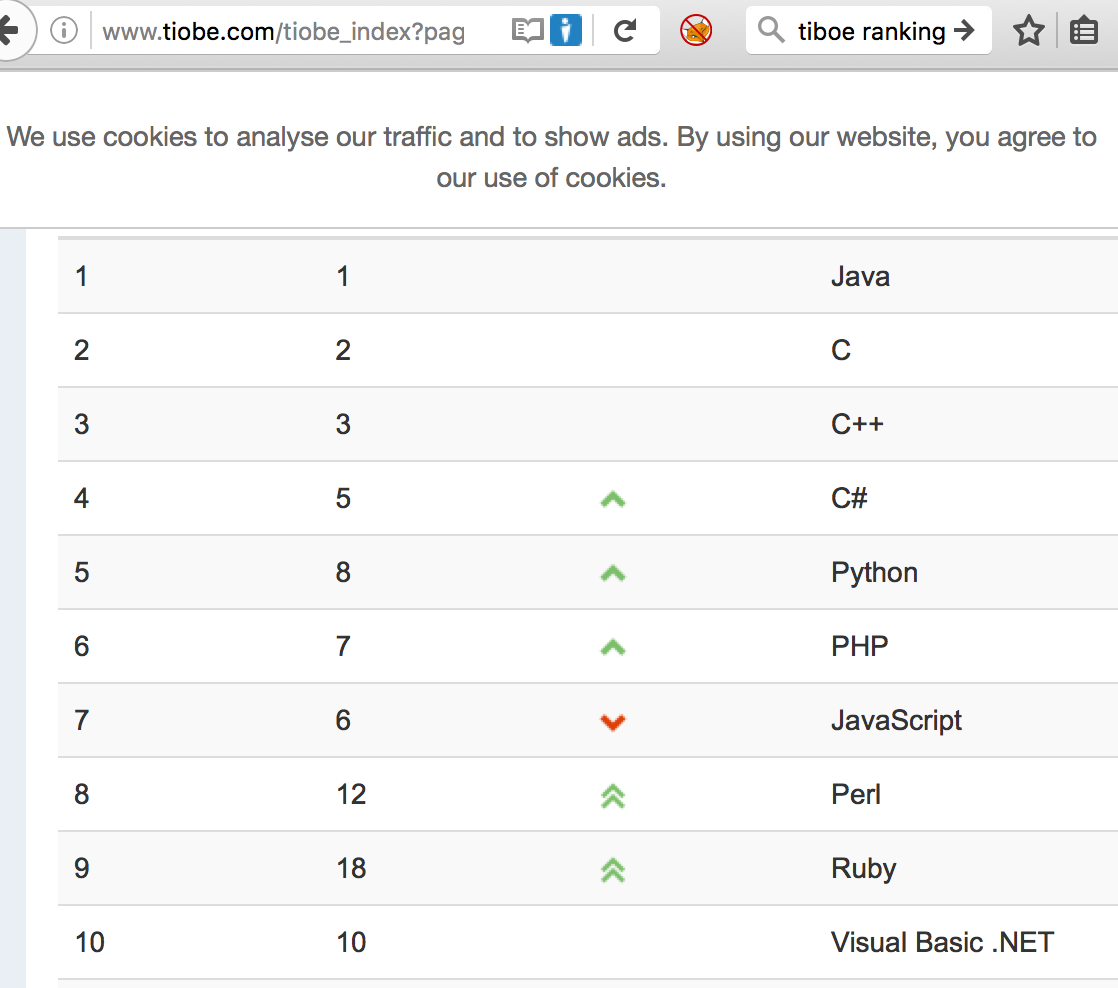
\includegraphics[width=0.9\linewidth]{Images/tiboe}
	\end{figure}
\end{frame}

\begin{frame}
	\huge ¿Que es Java?
\end{frame}

\begin{frame}{Lenguaje}
	\begin{figure}
		\centering
		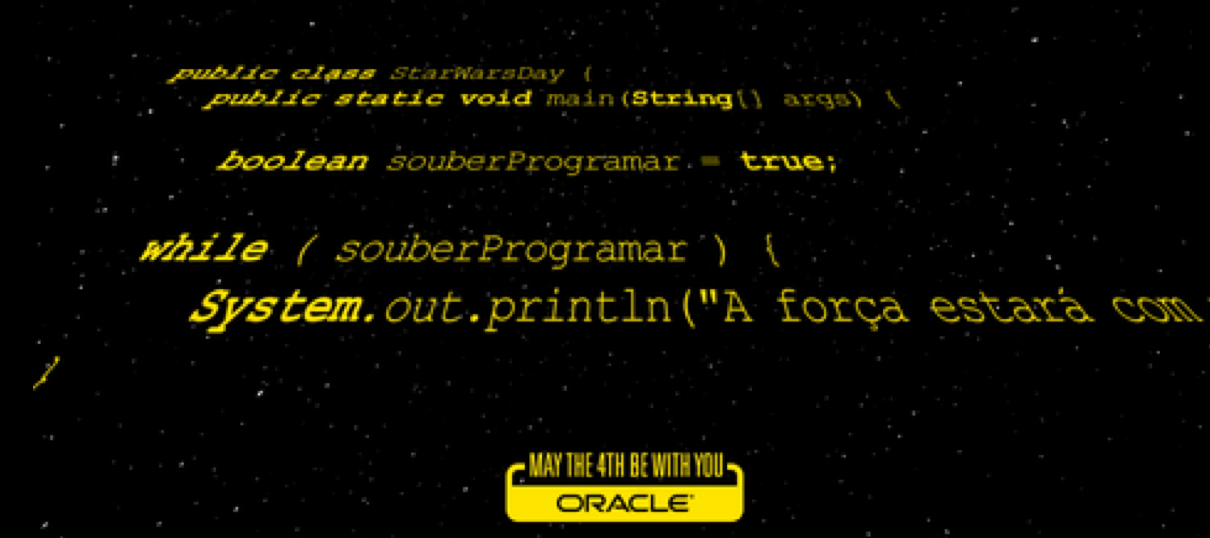
\includegraphics[width=0.9\linewidth]{Images/javalang}
	\end{figure}
\end{frame}

\begin{frame}{Maquina virtual}
	\begin{figure}
		\centering
		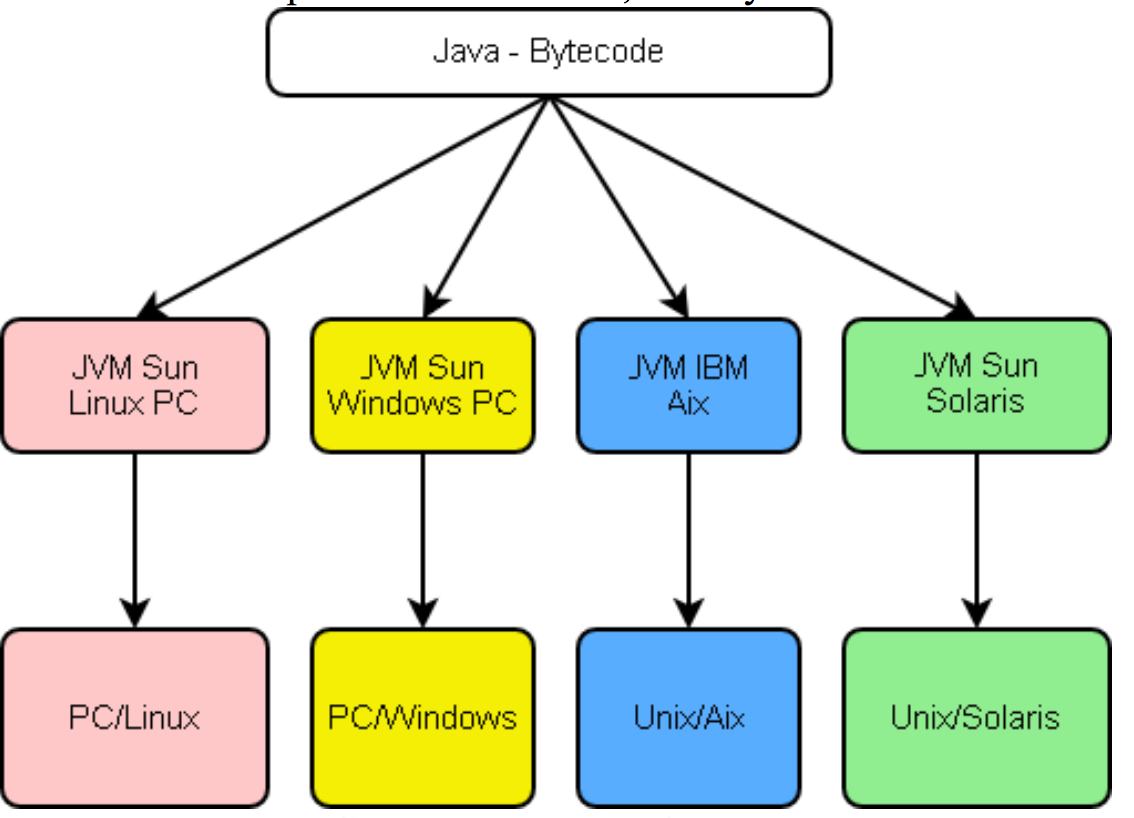
\includegraphics[width=0.9\linewidth]{Images/jvm}
	\end{figure}
\end{frame}

\begin{frame}{Muchas plataformas}
	\begin{figure}
		\centering
		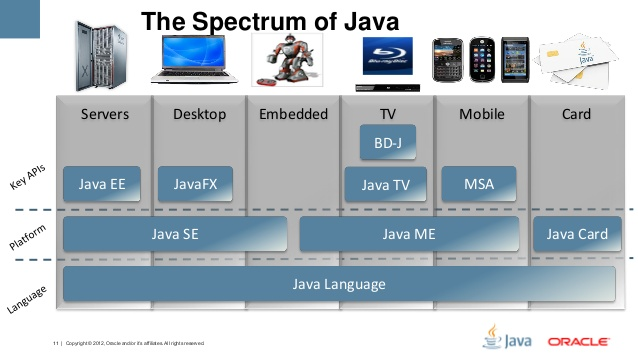
\includegraphics[width=0.9\linewidth]{Images/spectrum}
	\end{figure}
\end{frame}
\iffalse
\subsection{Framework}

\begin{frame}{Framework - Web}
	\begin{figure}
		\centering
		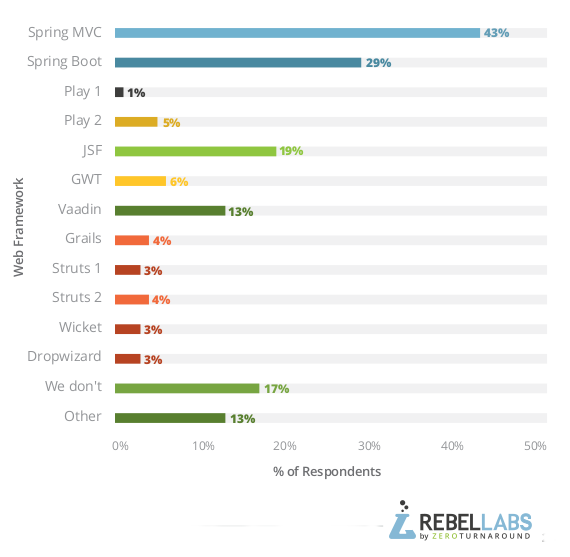
\includegraphics[width=0.9\linewidth]{Images/fwjava}
	\end{figure}
\end{frame}

\begin{frame}{Framework - Enterprise}
	\begin{figure}
		\centering
		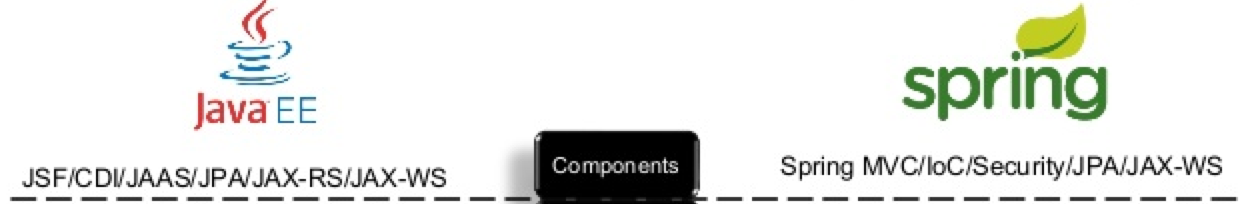
\includegraphics[width=\linewidth]{Images/javaeesp}
	\end{figure}
\end{frame}

\begin{frame}{Framework - Ligero}
	\begin{figure}
		\centering
		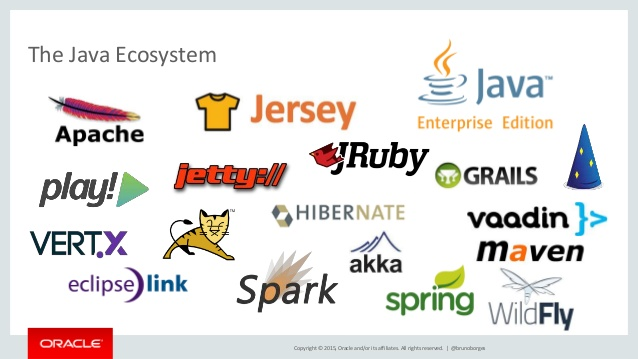
\includegraphics[width=0.9\linewidth]{Images/ecosystem}
	\end{figure}
\end{frame}

\begin{frame}{Framework - Embarcado}
	\begin{figure}
		\centering
		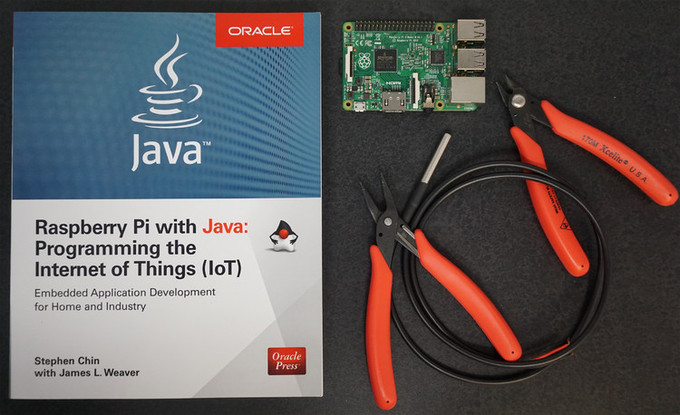
\includegraphics[width=0.9\linewidth]{Images/javapy}
	\end{figure}
\end{frame}

\begin{frame}{Framework - Movil}
	\begin{figure}
		\centering
		
\includegraphics[width=0.9\linewidth]{Images/android}
	\end{figure}
\end{frame}

\fi
\section{\faLock Seguridad en Java}
\subsection{Modelos}
\begin{frame}{Infosec}
\centering
\smartdiagram[bubble diagram]{Seguridad,
	Confidencialidad, Integridad, Disponibilidad}
\end{frame}

\begin{frame}{Seguridad}
\centering
\Tree [.Seguridad JVM Lenguaje Bibliotecas ]
\end{frame}

\subsection{JVM}
\begin{frame}{Seguridad}
\centering
\Tree [.Seguridad [.JVM Escritorio Applets Invasión ] Lenguaje Bibliotecas ]
\end{frame}


\subsection{Lenguaje}
\begin{frame}{Seguridad}
\centering
\Tree [.Seguridad JVM [.Lenguaje Tipado Punteros Scopes ] Bibliotecas ]
\end{frame}


\subsection{Bibliotecas}
\begin{frame}{Seguridad}
\centering
\Tree [.Seguridad JVM Lenguaje [.\textbf{Bibliotecas} Manual Frameworks Runtimes ] ]
\end{frame}


\begin{frame}{Bibliotecas}
¿Cual?
		\begin{itemize}
			\item Apache Shiro
			\item Spring Security
			\item OACC
			\item Picketlink
			\item Keycloak
			\item JGuard
			\item JACC
			\item SoteriaRI
		\end{itemize}
. . .
\end{frame}



\begin{frame}{Tecnologias Web}
\begin{columns}[T] % contents are top vertically aligned
	\begin{column}[T]{5cm} % each column can also be its own environment
		Render en servidor
		\begin{itemize}
			\item JSF (Icefaces, Primefaces)
			\item GWT
			\item JSP
			\item Servlets
			\item Vaadin
			\item Struts
			\item Spring MVC
		\end{itemize}
	\end{column}
	\pause
	\begin{column}[T]{5cm} % alternative top-align that's better for graphics
		Render en cliente
		\begin{itemize}
			\item Angular
			\item React
			\item Knockout (Oracle JET)
			\item Vue
		\end{itemize}
		\pause
		Servicios
	\begin{itemize}
		\item SOAP
		\item Rest
		\item RMI
	\end{itemize}
	\end{column}
\end{columns}
\end{frame}

\begin{frame}{Tecnología}
\begin{figure}
	\centering
	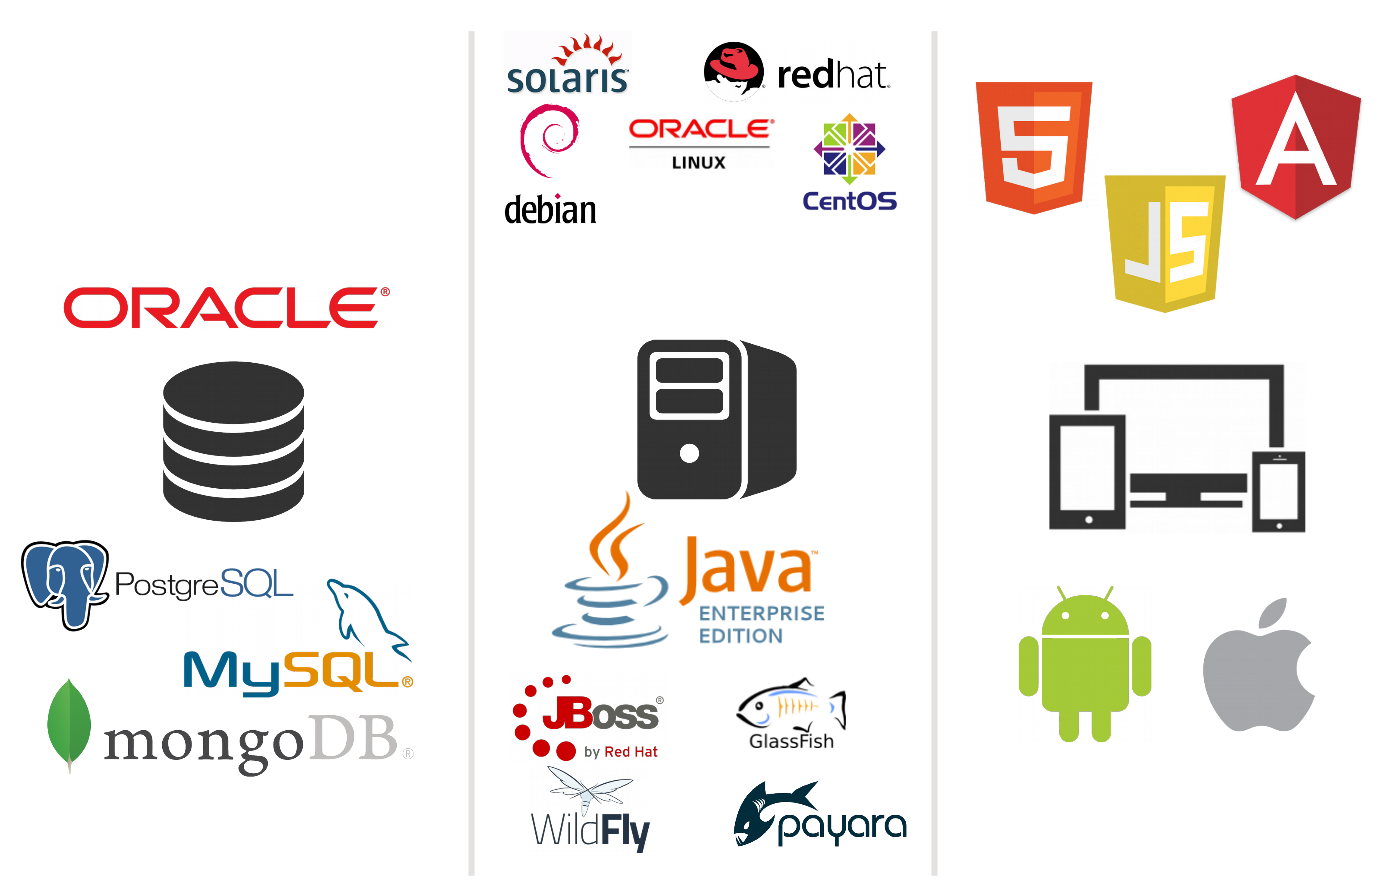
\includegraphics[width=\linewidth]{Images/tecno}
\end{figure}
\end{frame}


\begin{frame}{JavaEE 7}
\begin{itemize}
	\item API Rest - JAX-RS 2.0
	\item WebSocket - WebSocket 1.0, Servlet 3.1
	\item JSON - JSON API 1.0
	\item SOA, Microservices
\end{itemize}
\begin{figure}
	\centering
	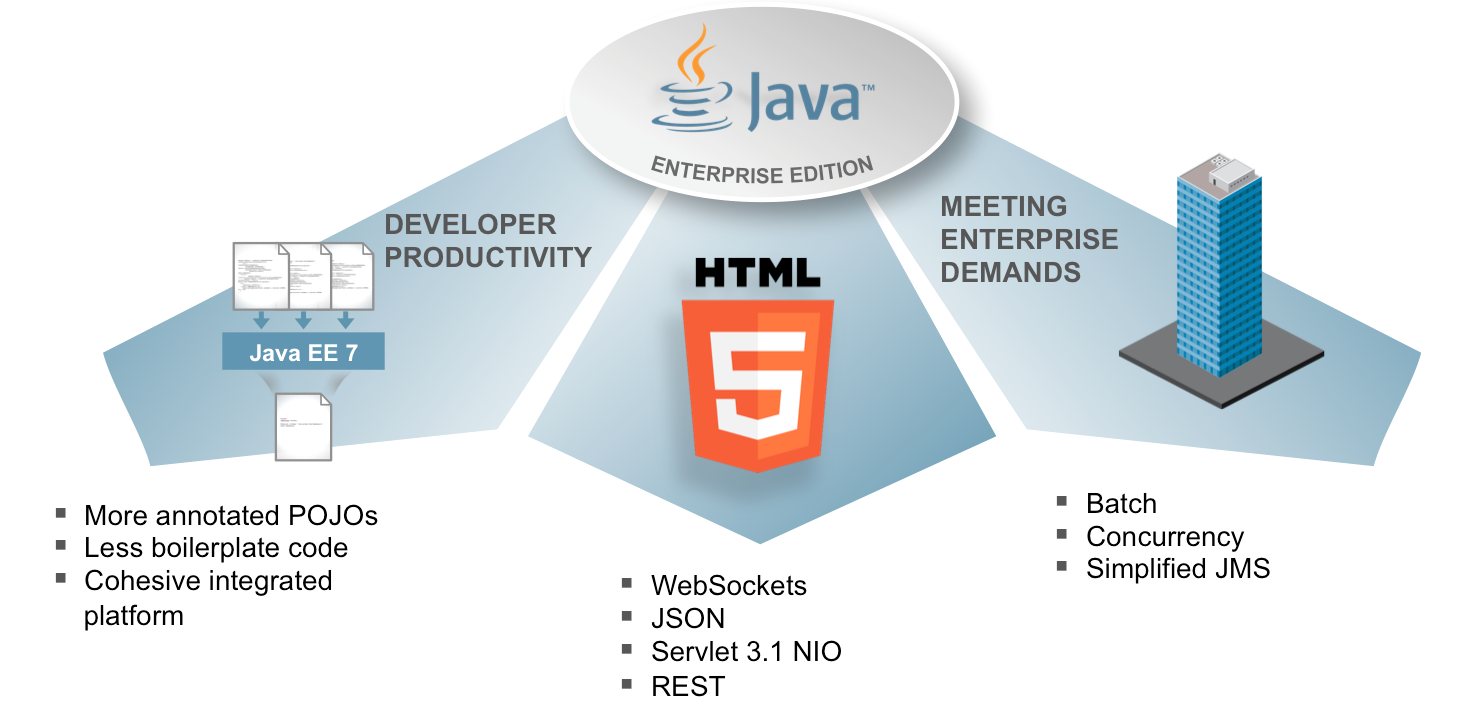
\includegraphics[width=0.7\linewidth]{Images/javaee7-theme}
\end{figure}

\end{frame}

\begin{frame}{JavaEE 7}
\begin{figure}
\centering
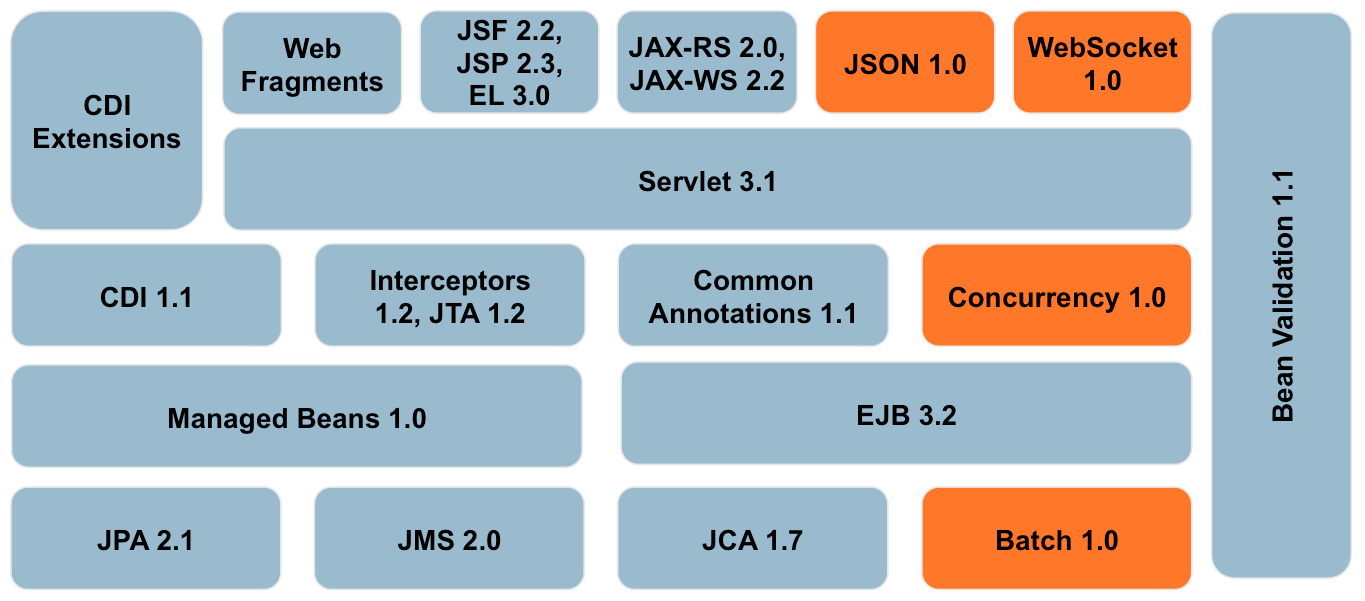
\includegraphics[width=0.9\linewidth]{Images/javaee7-pancake.png}
\end{figure}

\end{frame}


\begin{frame}{JavaEE 8}
	\begin{itemize}
		\item Mejor integración de JSF con CDI
		\item Mejor integración de JMS con CDI
		\item HTTP/2
		\item JSON-B
		\item Security
		\item JAX-RS Reactivo
	\end{itemize}
\end{frame}

\begin{frame}{JavaEE 8}
\begin{figure}
	\centering
	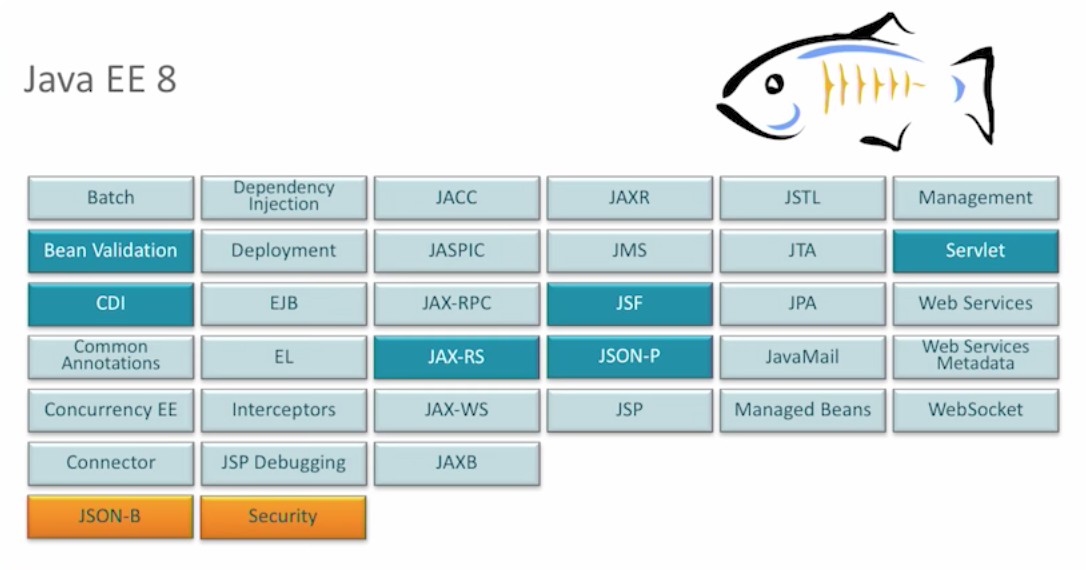
\includegraphics[width=0.9\linewidth]{Images/javaee8}
\end{figure}
\end{frame}


\section{EE vs OWASP Top 10}

\begin{frame}{Advertencia}
\begin{itemize}
	\item Visto en N desarrollos
	\item Un punto de inicio
	\item Informar
\end{itemize}
\end{frame}

\begin{frame}{JavaEE}
\begin{itemize}
	\item A1-Injection
	\item A2-Broken Authentication and Session Management
	\item A3-Sensitive Data Exposure
	\item A4-XML External Entities
	\item A5-Broken Access Control
	\item A6-Security Misconfiguration
	\item A7-Cross-Site Scripting (XSS)
	\item A8-Insecure deserialization
	\item A9-Using Components with Known Vulnerabilities
	\item A10-Insufficient Logging y Monitoring
\end{itemize}
\url{https://www.owasp.org/index.php/Top_10_2017-Top_10}
\end{frame}

\begin{frame}{JavaEE}
\begin{itemize}
\item \textbf{A1-Injection}
\item \textbf{A2-Broken Authentication and Session Management}
\item \textbf{A3-Sensitive Data Exposure}
\item A4-XML External Entities
\item \textbf{A5-Broken Access Control}
\item \textbf{A6-Security Misconfiguration}
\item A7-Cross-Site Scripting (XSS)
\item \textbf{A8-Insecure deserialization}
\item \textbf{A9-Using Components with Known Vulnerabilities}
\item A10-Insufficient Logging y Monitoring
\end{itemize}
\url{https://www.owasp.org/index.php/Top_10_2017-Top_10}
\end{frame}


\begin{frame}{JavaEE - A1 - Injection}
Problemas y causas comunes
\begin{itemize}
	\item Concatenación de Strings en SQL
	\item Datos mal intencionados a aplicaciones
	\item Manipulación data stores
	\item Escalar privilegios
\end{itemize}

Sugerencias
\begin{itemize}
	\item JAMAS y NUNCA concatenar parametros
	\item Siempre utilizar mecanismos de \texttt{sanitizing}
	\item Parchar con OWASP ESAPI
	\item JDBC y JPA soportan de serie sanitizing si no se concatena
	\item Bean Validation en parametros
\end{itemize}
\end{frame}


\begin{frame}{JavaEE - A2-Broken Authentication and Session Management}
Problemas y causas comunes
\begin{itemize}
	\item Implementación de solución manual vs frameworks
	\item Falta de políticas 
	\item Entrenamiento en la plataforma
	\item Comunicación y/o autenticación via http
\end{itemize}

Sugerencias
\begin{itemize}
	\item Forzar https
	\item Utilizar adecuadamente los ciclos de vida de la plataforma (singleton != stateless != statefull) y cache
	\item No implementar en base a interceptores
\end{itemize}
\end{frame}



\begin{frame}{JavaEE - A3-Sensitive data exposure}
Problemas y causas comunes
\begin{itemize}
	\item Guardar datos sin cifrar
	\item Datos con cifrado "debil", AKA cifrado propio
	\item Transmitir credenciales via http
	\item Transmisión de excepciones completas a front-end
\end{itemize}

Sugerencias
\begin{itemize}
	\item Identificar con un checklist los datos sensitivos
	\item Evitar cifrado de dos vías a menos que sea necesario
	\item Evitar transmisión de llaves
	\item Verificar código auto generado (excepciones)
\end{itemize}
\end{frame}


\begin{frame}{JavaEE - A5-Broken Access Control}
Problemas y causas comunes
\begin{itemize}
\item Implementación de solución manual vs frameworks
\item Falta de políticas 
\item Escalar privilegios
\item Comunicación y/o autenticación via http
\end{itemize}

Sugerencias
\begin{itemize}
\item Forzar https
\item Implementación RBAC de application server
\item Implementación RBAC de framework
\item Entender el modelo de JAAS y SoteriaRI
\end{itemize}
\end{frame}



\begin{frame}{JavaEE - A6-Security Misconfiguration}
Problemas y causas comunes
\begin{itemize}
	\item Configuración por defecto de applicaction server
	\item Configuración por defecto de SO
	\item Configuración \texttt{relajada} de capa de transporte
\end{itemize}

Sugerencias
\begin{itemize}
	\item Configurar siempre el SO destino
	\item Proteger Glassfish
	\item Firewall
	\item RBAC
	\item Evitar certificados autofirmados en entornos no controlados
	\item JVM tipo \texttt{server}
\end{itemize}
\end{frame}


\begin{frame}{JavaEE - A8-Insecure deserialization}
Problemas y causas comunes
\begin{itemize}
	\item Self made frameworks
	\item No validation
\end{itemize}

Sugerencias
\begin{itemize}
	\item Evaluar si no vale la pena utilizar un software listo
	\item Bean validation
\end{itemize}
\end{frame}


\begin{frame}{JavaEE - A9-Using components with known vulnerabilities}
Problemas y causas comunes
\begin{itemize}
	\item Difícil dar seguimiento a los lanzamientos
	\item Frameworks muy nuevos o muy viejos
	\item No seguir las notas del lanzamiento
\end{itemize}

Sugerencias
\begin{itemize}
	\item Actualizar el app server con el calendario de lanzamiento
	\item Suscripción a mailing list/foros
	\item Servicios tipo Bintray
	\item Servicios de análisis estático (Sonar)
\end{itemize}
\end{frame}

\begin{frame}{JavaEE - Bonus-APIs sin proteger}
Problemas y causas comunes
\begin{itemize}
	\item Combinación de broken auth, broken access control o security misconfiguration
	\item No hay nada
	\item Especialmente grave en rich clients
\end{itemize}

Sugerencias
\begin{itemize}
	\item Verificar código auto generado
	\item Programar en modo \texttt{deny all}
\end{itemize}
\end{frame}


\subsection{Apache Shiro}

\begin{frame}{Apache Shiro}
\begin{figure}
	\centering
	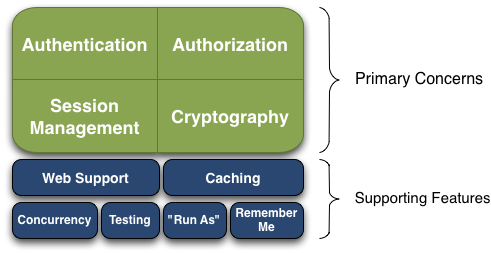
\includegraphics[width=0.7\linewidth]{Images/ShiroFeatures}
\end{figure}

\end{frame}


\begin{frame}{Apache Shiro}
\begin{itemize}
	\item Java Authentication and Authorization Service - JAAS
	\item RBAC
	\item Autenticación
	\item Autorización
	\item Cifrado
\end{itemize}
\end{frame}
\begin{frame}{Apache Shiro - Taxonomia}
\begin{itemize}
	\item Permission
	\item Principal (generic attribute)
	\item Subject (user)
	\item Credential
	\item Realm
	\item Role
	\item Session
\end{itemize}
\end{frame}

\section{Fin}

\begin{frame}{Gracias}
\begin{itemize}
	\item me@vorozco.com vorozco@nabenik.com
	\item http://vorozco.com
	\item http://github.com/tuxtor/slides
\end{itemize}
\begin{center}
	
\includegraphics[width=0.1\linewidth]{Images/cclogo}
	\\
	This work is licensed under a Creative Commons Attribution-ShareAlike 3.0 Guatemala License.
\end{center}
\end{frame}
\end{document}

